	\documentclass{llncs}
	\usepackage{llncsdoc}
	\usepackage[noend]{algpseudocode}
	\usepackage{subfig} 
	\usepackage{graphicx}
	\usepackage{frame, caption}
	\usepackage{amsmath}
	\usepackage{eulervm}
	\usepackage{fontenc}
	\usepackage{mathrsfs}
	\usepackage{multirow, enumitem, longtable, rotating}
	\usepackage{array}
	\usepackage[rflt]{floatflt}
	\usepackage{makecell}	
	\usepackage{xcolor, soul}
	\sethlcolor{yellow}	
	\usepackage{floatrow}

	\setlength\extrarowheight{3pt}
	% Table float box with bottom caption, box width adjusted to content
	\newfloatcommand{capbtabbox}{table}[][\FBwidth]
	
	\begin{document}
	\title{\vskip -10pt Dominance in dialogue of collaborative negotiation}
	
	\author{Lydia Ould Ouali\inst{1}, Charles Rich\inst{2} \and
		Nicolas Sabouret\inst{1} }
	
	\institute{LIMSI-CNRS, UPR 3251, Orsay, France \\
		Universit\'e Paris-Sud, Orsay, France \\
		\email{\{ouldouali, nicolas.sabouret\}@limsi.fr}
		\and
		Worcester Polytechnic Institute\\ Worcester, Massachusetts, USA\\
		\email{rich@wpi.edu}
	}

	\maketitle
	
	\begin{abstract}
		This paper presents a model of conversational agent that can deploys different strategies of negotiation based on the social power it wants to express for the user. This model is based on three principles of collaborative negotiation from the literature in social psychology. We show that this principles are correctly perceived by a human observer: the social behavior of the agent is made visible through its dialogue strategy.
	\end{abstract}
	
	\section{Introduction}
	As artificial conversational agents become more and more popular, they became capable to hold a conversation with a human user and potentially collaborate with the user in order to achieve a common objective. For example, artificial tutors collaborate with students [ref], or a companion agents can help elderly to follow a specific diet \cite{kidd2005sociable}. In this context, the user(s) and the agent have to negotiate in collaborative manner about the way to achieve the common task. This is called \emph{collaborative negotiation}. Unlike adversarial negotiation \cite{traum2008multi}, collaborative negotiation assumes that each participant is driven by the goal of finding a trade-off that best satisfies the interests of all the participants as a group, instead of one that maximizes his own interest\cite{sidnerartificial,chu1995response}.
	
	Moreover, previous research has shown that people tend to respond to computers as social actors \cite{bickmore2005establishing}. This led the IVA community to study the psychosocial relationship between the user and the agent during their interaction: a growing body of research is investigating the use of appropriate social behavior for virtual agents in different roles and types of user-computer relationship \cite{bickmore2005s,bickmore2005establishing,kidd2005sociable}. In the context of human-human communication involving negotiation, social psychology and communication \cite{dunbar2005perceptions,de1995impact} investigated the impact of social relations and emotion on the negotiation. They proved that  \emph{interpersonal power} directly affects the strategies of negotiators. Therefore, in order to build intelligent conversational agents that conduct good collaborative negotiations, it is very important to allow them to adapt their negotiation strategies to different levels of interpersonal power. [Traum et al. studied this question in the context of adversarial multi-party negotiation. We consider the case of collaborative one-to-one dialogue.]
	
	In this paper, we present a model of conversational agent that can deploys different strategies of negotiation based on the social power it wants to express for the user. In the next section, we discuss existing works on interpersonal power in the domain of social psychology and affective computing. Section 3 presents the negotiation model, based on a set of utterance types and a model of preferences. It implements three principles of collaborative negotiation from the literature in social psychology. In section 4, we present an experiment conducted with two virtual agents and we show that these principles are correctly perceived by a human observer.	
	
	\section{Related works}
	The notion of social power has been widely studied in the fields of interpersonal communication and psychology \cite{kecskes2013research}. It can be defined as the capacity to produce intended effects and ability to influence the behavior of other person in the conversation \cite{dunbar2005perceptions}. In the context of communication, power is a dyadic variable that takes place during the dialogue, where the interlocutor who exerts power is viewed as \textit{dominant}, while the interlocutor with low power's behaviors is viewed as \textit{submissive}. 
% where one individual's attempt of control is necessarily acquainted by the partner in the interaction.\cite{dunbar2005perceptions}

	Behaviors related to power can contribute either positively or negatively to the dialogue. Positive contributions include keeping the conversation going, making quick decisions, etc. Negative contributions include not considering the partner (\emph{e.g.} not giving the occasion to express his opinion), appearing offensive, etc. \cite{zablotskaya2012relating}. In our work, we focus on negotiation dialogues, for which several researchers already proved the impact of power on the negotiation \cite{van2006power}.
	
	\subsection{Behaviors of power in dialogue}
	\label{domDialogue}
	During a conversation, power can manifest through verbal and nonverbal behaviors.	
	At the nonverbal level, a wide range of behaviors have been associated with the relation of power in kinestesic behaviors (facial expression, body movements and gestures) and voice (speaking duration, speaking intensity, voice control and pitch) \cite{burgoonnonverbal}.
	
	Verbal behaviors of power in the dialogue are related to the type of \textit{strategies} that individuals choose in order to take control of the other especially during a negotiation. A considerable body of research has documented the effects of power on negotiation behaviors and outcomes. De Dreu demonstrated that \cite{de1995impact} dominant negotiators have higher aspirations, demands more and concede less. Galinsky \cite{galinsky2003power} affirms that power increases the action orientation: dominant negotiators control the flow of the negotiation. In addition, high power increase task orientation and goal-directed behavior. \cite{giebels2000interdependence} shows that this leads dominant negotiators to end up with the larger share of the pie.
	
	Furthermore, power affects the way that negotiators gather information about their partners \cite{de2004influence}. Submissive negotiators have a stronger desire to develop an accurate understanding of their negotiation partner, which would lead them to ask more \emph{diagnostic} rather than \emph{leading} questions.
	
	It was also shown that dominant negotiators are self-centered and tend to not pay attention to the preferences of submissive negotiators \cite{fiske1993controlling,de1995impact}.
	%					 The idea is that high-dominant individuals have many resources and can often act at will without serious consequences, while submissive individuals, have to be more careful because they are more dependent on other people. In addition, they are motivated to gain or regain control over their outcomes by paying close attention to the people on whom they depend.
	%					

	In our work, we use a text-oriented dialogue system and we therefore focus on the verbal behaviors.  Our goal is to make visible \emph{the strategies} deployed during the negotiation depending on the power. In order to implement these different behaviors, we extracted three principle related to the relation of power that impact strategies of negotiation:
	\begin{enumerate}
	\item \textbf{Self Vs Other:} Submissive negotiators consider the preferences of other in the negotiation, whereas dominant negotiators  are self-centered and only interested by satisfying their own preferences. \cite{fiske1993controlling,de1995impact}
	
	\item \textbf{Representation of demands:} Dominant negotiators show a higher level of demand than the submissive ones. In addition,  Submissive negotiator's demand decrease over time, and tends to make larger concessions than dominant negotiators. \cite{de1995impact}
	
	\item \textbf{Control the flow of the negotiation:}
	Dominant negotiators tend to make the first move \cite{magee2007power}. In addition, they take the lead of the negotiation. Otherwise, submissive negotiators aim to construct an accurate model of other preferences, which lead them to ask more questions about other preferences rather than keeping the negotiation going (makes proposals). \cite{gather-info}
	
	\end{enumerate}
	%	We will present in the next section the decision model based on the behaviors of power. 
	%						\item Based on Carsten, De Dreu and Van Kleef demonstrate that high power negotiators are high in their propensity to negotiate relative to participants with low power. (leading individuals to focus on the rewards available to them in situations and to bargain forgreater rewards than were initially offered to them.)			
	
	\subsection{Power in affective computing}
	Different models enabling conversational agents to exhibit social power behaviors through their verbal and nonverbal behavior have been proposed. 
	
	Most of the existing works investigate the nonverbal behavior of power. For instance, \cite{lance2008relation} proposed an animated virtual agent with a gaze model for emotional expression based on Mehrabians PAD model \cite{mehrabian1996analysis}. They demonstrated that power was associated to a raised head and fast movements. These results were also \cite{mignault2003many} works.
	 Further on, \cite{gebhard2014exploring,callejas2014computational} demonstrated that head-tilt as well as the use of spacial movements is related to power and submissive perception. 
	  
	\par Other works investigated the perception of power combined to other social aspects. For instance,\cite{strassmann2016effect} investigate the perception of nonverbal behaviors of virtual agents with a focus on power and cooperation. On the same vain,  \cite{bee2010bossy} combines in their model the perception of nonverbal behaviors from the PAD model \cite{mehrabian1996analysis} with verbal behaviors related to personality traits from the big five model.
	 They demonstrated that the linguistic personality traits influence the perception of power. Reciprocally, gaze-based power influences the perception of personality traits.
	
	 
	These researches differ from ours in two main points. First, they model the power as an individual trait, while in our research, we consider the power as an interpersonal relation, which means that it takes place between the agent and the user(dyadic trait). 
	Second, most of theses research focused on nonverbal behaviors of power, while we are interested in the verbal behaviors. Moreover, we aim to study the effect of power at a decisional level, where we investigate how power affects the strategies of negotiation in dialogue.
	
	
	\section{Model of negotiation based on the relation of power}
	In this section, we present our model of dialogue of negotiation of preferences.	
	First, we present the domain of model that represent the agent's preferences and the representation of topics of negotiation. Second, we present the implementation of the principles of behaviors of power in negotiation (see section \ref{domDialogue}).

	\subsection{Domain model}
	The overall goal of a negotiation in our dialogue model is to choose an \textbf{option} in a set of possible options for a given topic. For instance, on the topic ``Restaurant'', we have a set of options: ``Chuck's cake'', ``Ginza''\ldots 
	 Let $\mathcal{O}$ be the set of options, and $V$ be the set of available options, such that option :$ V\rightarrow O$. For example, V is the set of restaurants that are mutually known to the interlocutors. 
		
	\par To be able to compare these options, interlocutors base their evaluation of each option on a set of \textbf{criteria} that reflect options characteristics. We consider a sequence of criterion sets $C_1, C_2, ..., C_n$ such as options set are defined as the cross-product:
	$O = C_1 \times C_2 \times \ldots C_n$.
	
	Furthermore, each criterion has to be measurable, in the sense that it must be possible to rate an option. Therefore, $\forall$ \emph{c $\in C_i$},  we note \emph{$V_i$} its  domain of values mutually knowns by interlocutors. For example, the domain values of the criterion cuisine is noted $\emph{V}_{cuisine} = \{chineese, italian, \ldots\}$.
%	For example, for restaurants, the criteria might be:
%	
%	Cuisine = \{Chinese, French, ...\} /Atmosphere = \{quiet, lively, ...\}. 
%	
%	and a restaurant options might be: 
%	
%	$[Chinese, cheap, lively]$. / $[Japanese, expensive, quit]$.   
%	%\item $[Chinese, expensive, lively]$.
%	%					\item $[French, cheap, quit]$.  
%	%					\item $[French, expensive, quit]$.   
%	%					\item $[Chinese, expensive, lively]\ldots$ 
	\subsection{Self model} 
		In order to allow the agent to negotiate about its preferences, we define a model about agent's preferences for each criterion of the topic. Preferences are represented as partial orders on the criterion sets. The preference relation on the criterion set $C_i$ is denoted by $\prec_i$.			
		Let $\prec$ denotes the sequence of preferences $\{ \prec_i, \prec_2, ..., \prec_n\}$.
	
		Using the set of binary preferences$\prec_i$, an agent is able to rate he likes a value $v \in V_i$ compared to other values in $V_i$. we denote a function \emph{Satisfaction} which is normalized to [0,1] that evaluates an element of a criterion set relative to the corresponding preference relation.

	\begin{equation}
	sat(v, \prec_i) =	1 - \left( \frac{|\{d : d \neq c \  \wedge \ (v \prec_i d)\}| }{( |V_i| - 1 )}\right)
	\end{equation}
	
	
	Satisfaction is generalized to options as a weighted sum.
	For $o \in O$ and where $o_i$ is the i-th element of $o$ and $\prec_i$ the i-th element of $\prec$.
	\begin{equation}
	sat(o, \prec) = \frac{\sum_{i}^{n} sat(o_i, \prec_i) }{n}
	\end{equation}
	
	\subsection{Dialogue model}
		Negotiators communicate during the negotiation via utterances. We generated nine types of utterance based on Sidner work. \cite{sidnerartificial}. 
		
		\begin{table}[h]
			\begin{tabular} {|p{2.5cm}|p{3.5cm}|p{6cm}|}
				\hline
				Utterance type & input & Format \\
				\hline
				StatePreference & $c \in V_i$ & I (don't) like $c$.\\
				\hline
				 \multirow{2}{*}{AskPreference} &$c \in V_i$ & do you like $c$ ?\\
				 \cline{2-3}
				 & $c \in C_i$ & What kind of $c$ do you like ? \\
				 \hline
				 Propose & $p / p\in V_i \vee p \in V$ & Let's go to $p$. \\
				 \hline
				 Reject & $p / p\in V_i \vee p \in V$ & I'd rather choose  something else \\
				 \hline
				 RejectPropose & $r, p / r,p\in Vi \vee r,p \in V $ & I don't want to go to $r$. Let's rather go to $p$ \\
				 \hline 
				 RejectState & $ p,c / p,c\in Vi \vee p \in V$ &  I don't like $c$, let's choose something else \\
				 \hline
				 Accept& $p / p\in V_i \vee p \in V$& Okay, let's go to $p$	 \\
				 \hline
				 AcceptPropose & $a,p / a,p\in Vi \vee a,p \in V $ & Okay. Let's go to $p$\\
				 \hline
			\end{tabular}
			\caption{The list of possible utterances in the model of dialogue}
		\end{table}
	
	In order to produce coherent dialogues, the agent keeps track of the different states of the dialogue updated after each move. 
	The negotiation have to take into account each criterion of the discussed topic. For example, in a negotiation on restaurants, speakers might negotiate about the type of \textit{cuisine}, and the \textit{ambiance} to choose.  
	
	First, the agent processes a model about the other interlocutor's preferences during the negotiation (\textit{i.e. model of other}). Let the collection of $A_i \subseteq C_i$ be the criterion values that are satisfiable to the other, and $U_i \subseteq C_i$ be the criteria values that are not.  We assume $A_i \cap U_i = \emptyset$.  Note that some values are thus unknown.
	
	Then the satisfiability of a criterion $c \in C_i$ is a function normalized to [0,1] and defined as follows.
	\begin{equation}
	other(c, A_i, U_i)= \left\{\begin{array}{ll}
	1	 & \mathrm{if\ }  c \in A_i\\
	0    & \mathrm{if\ }c \in U_i\\
	0.5	 & \mathrm{otherwise}
	\end{array}\right.
	\end{equation}
	
	This function is generalized to option $o \in O$ as a weighted sum.
	
	\begin{equation}
	other(o, A, U) = \frac{ \sum_{i}^{n} other(o_i, A_i, U_i) } {n}
	\end{equation}
	
	Second, information about the \textit{negotiation state} are processed. \\
	We note  $s_i, p_i, t_i, r_i \subseteq C_i$, respectively, the criterion values stated by the agent in the dialogue, values which have been proposed, values which have been accepted and the values rejected in the negotiation. 
		
	Similarly, we define the same structure of proposals for the options called $P, R, T$
	
	\subsection{Decision based on power in negotiation}
	\label{decision}
	We extracted from social psychology works three mains principles related to the relation of power which affects negotiators strategies and behaviors (see section \ref{domDialogue}). We present in this section, the formal theory built for each principle. 
	
	\subsubsection {Self vs other}
		It was proved that dominant negotiators are self-centered, whereas submissive negotiators care about fairness and the well being of the other negotiator. Therefore, we can conclude, that the higher the power gets,the higher a negotiator give weight to the satisfaction of its preferences.
	
		Let  $pow \in [0, 1] $ denotes the agent's perception of its relationship of power. It is a constant for a given agent in a given relationship.
	The weight that an agent gives to its self-satisfaction relative to	the satisfaction of the other is a function normalized to 	[0,1] of its power, defined as below.
	%time-varying
	\noindent
	\begin{minipage}{0.5\textwidth}
		\begin{equation}
		self(pow, t) = \left\{\begin{array}{ll}
		pow & \mathrm{if\ } (t \leq \tau)\\
		max(0, pow - (\frac{\delta}{pow} . (t - \tau))) & \mathrm{otherwise}
		\end{array}\right.
		\end{equation}
	\end{minipage}
	 \begin{minipage} {0.5\textwidth}
		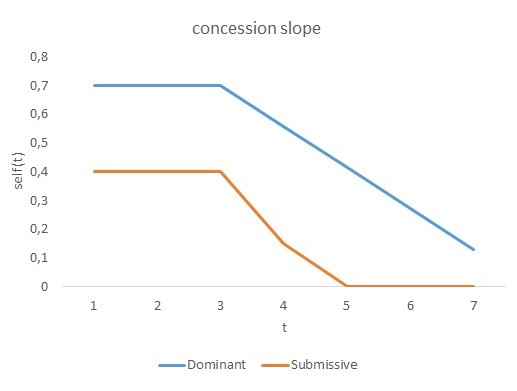
\includegraphics[width=\linewidth,keepaspectratio=true]{graphs/slope.jpg}
	 \end{minipage}
	
	where is $t \geq 0$ is the number of open or rejected proposals and $\tau > 0$ and $\delta > 0$
	are parameters of the theory in general and are initially assumed to
	be 2 and 0.1, respectively.
	
	Let be	$\{V' \subset V$ / $\forall v \in V', acc(v,t) = true\}$ be the list of agent's acceptable values. 
	
		In the context of collaborative negotiation, the value of a proposal should be \textit{tolerable} for both interlocutors. Therefore, in addition to self preferences, the agent should considers other's preferences when proposing a value, with respect to the weight it gives to its preferences.
	%	We define a tolerance function of a criterion $c \in C_i$ as a function normalized to [0,1]:
	\begin{equation}
	 tolerable(pow, t, c, \prec, A, U) = self(pow, t) . sat(c, \prec_i)  +  (1 - self(pow, t)) . other(c, A_i, U_i)
	\end{equation}
	
	\begin{equation}
	tolerable(pow, t, o, \prec, A, U) = \frac{ \sum_{i}^{n} tolerable(pow, t, o_i, \prec_i, A_i, U_i) } {n}
	\end{equation}
	
	\subsection{Level of demand and concessions}
		Based on the second principle, dominant negotiators are more demanding than the submissive ones. Therefore, the acceptability of a value $c \in V_i$  is relative to the weight an agent gives to its self satisfaction:
				\begin{equation}
				acc(c, t) = sat(c, \prec_i) \geq  \beta . Self(t).
				\end{equation}
				
				This function is generalized to option $o \in O$:
				\begin{equation}
				acc(o, t) = sat(o, \prec) \geq  \beta . Self(t)
				\end{equation}
	
		
		Furthermore, we represent the notion of concession, by making the agent decreases the weight that of its self satisfaction during the negotiation. Indeed, we place our dialogue model in the context of \textit{collaborative negotiation}. Therefore, we aim to make the negotiation succeed which lead the negotiators to make concessions if the negotiation is not converging. We, thus define a \emph{"concession curve"} see figure(), where Self(t) decreases when the number of open or rejected proposals during the negotiation increase (i.e the negotiation is not converging).
		

			

	\subsection{Lead of the negotiation}
		The third principle relates that the dominant negotiators initiate the negotiation. Therefore, we model the dominant agent to always start the negotiation. In addition, dominant negotiator tend to lead the negotiation. Therefore, we model the dominant agent to focus on keeping the negotiation going by choosing \emph{negotiation moves}.  \footnote{\emph{negotiation moves:} Propose, Reject, Accept, RejectPropose, AcceptPropose}.
		In the opposite, a submissive negotiator aim to build an accurate model of other preferences in order to take the fairest decision in the end. Therefore, we made submissive negotiator to focus more on \emph{Statement moves}. \footnote{\emph{Statement moves}: StatePreference, AskPeference, RejectState}
		We present in table \ref{utt} the possible utterance responses and their applicability conditions. Note that each line (utterance) assumes that the previous ones are already not applicable.
	%This can be a many-to-one function, e.g., there could be two restaurants with same criteria.		
	
	% We name this function 	$ chooseUtterance(dom, t, V, \prec, A, U)$ 
	
	
	\begin{table}[t]
	\centering
	\begin{tabular}{|p{.45cm}|p{3cm}|p{8cm}|}
	\hline
	\parbox[t]{2mm}{\multirow{5}{*}{\rotatebox[origin=c]{90}{\textbf{pow  $>\pi$}}}}&\textbf{Utterance type} & Condition \\
	\cline{2-3}
	&Negotiation success & $\exists o \in T   \lor o \in P$ /  $acc(o,t) = true$ \\
	\cline{2-3}
	& Negotiation failure & $ \forall o \in O, acc(o,t) = false$\\
	\cline{2-3}
	& State & $type(u^{-1}) = AskPreference \land n < \alpha$ \newline- $n$ the number of successive statement moves \newline -$u^{-1}$ is the previous utterance.\\
	\cline{2-3}
	& AcceptPropose & $\exists c \in P_i$ / $acc(c,t)= true$ \\
	\cline{2-3}
	& RejectPropose & $\exists c \in P_i$ / $acc(c,t)= false$ \\
	\cline{2-3}
	& Propose & Otherwise  \\
	
	\hline
	\end{tabular}

	\begin{tabular}{|p{.45cm}|p{3cm}|p{8cm}|}
	\hline
	\parbox[t]{2mm}{
	\multirow{5}{*}{\rotatebox[origin=c]{90}{ \textbf{pow  $ \leq \pi$}}}} & \textbf{Utterance type} & \textbf{Condition} \\
	\cline{2-3}
	& Negotiation success &  $\exists o \in T$ \\
	\cline{2-3}
	& Accept & $\exists c \in P_i$, $acc(c, t)=true   \lor \exists o \in P$ ,  $acc(o, t) =true$ \\
	\cline{2-3}
	& RejectState & $ (\exists c \in P_i, acc(c, t)= false  \lor \exists o \in P ,  acc(o, t)=false)  \land (t<\tau$).\\
	\cline{2-3}
	& Propose & $\exists c$/$(other(c, A_i, U_i)  = 1  \land acc(c, t)=true) \lor
	\newline   (\forall c \in C_i$,  $c \in T_i$)\\
	\cline{2-3}
	& Ask &  $(t> \tau, \land \exists c \in P_i /$
	$ acc(c, t)=false)\lor$ \newline $(\forall c \in C_i,other(c, A_i, U_i)=0.5)$\\
	
	\cline{2-3}
	
	& State & $(type(u^{-1}) = AskPreference) \lor$
	\newline $(\exists x,other(x, A_i, U_i) \not = 0.5) \lor$  $ (\exists C \in \mathcal{C}, A_i(C) = Unkown)$
	\\
	\cline{2-3}
	& Propose & Otherwise \\
	\hline
	\end{tabular}
	\caption{Conditions to choose an utterance type}
	\label{utt}
	\end{table}

	\subsection{Summary of general parameters }
	\begin{itemize}[noitemsep]
	
	\item $\pi \in $[0,1] : boundary between submissive and dominant used in
	choosing an utterance type
	%		\item $\beta$:  a value that represent the minimum score that a value has to get to be positively satisfiable to the agent preferences in the negotiation. Note that $\beta = const \times self(dom,t)$.
	\item $\tau > 0$ : the minimum number of open or rejected proposals before concession begins
	\item $\delta > 0$ : parameter in slope of concession curve.
	\item $\alpha> 0$: the maximum number of successive statement moves.
	
	
	\end{itemize}
	
	
	
	
	
	\section{Evaluation}
	
	We built a conversational agent able to deploy strategies of negotiation based on its interpersonal relationship of power. In order to validate our model, we conducted a perceptual study in which participants had to determine the behaviors of two agents generated using our model. 
	
	\subsection{Study design}
	We implemented two conversational agents (\textit{speaker a} and \textit{speaker b}) which have to negotiate about a social topic of "negotiation about a restaurant where to have dinner".
	We generated a set of dialogues where we manipulated two conditions. First, the initial value of the power \textbf{pow} (see section \ref{decision}). 
	Speaker a will adopt a dominant negotiator's behaviors, while \textit{speaker b} will behave as a submissive negotiator. Therefore, power of \textit{speaker a} is initiated $pow>\pi$, complementarity \textit{speaker b} is initiated $ pow\leq \pi$.
	
	
	The second condition involved varying the initial preferences of both agents. We used the metric of Kendall distance \cite{bra2013Kendall} in order to compute the distance between two preferences sets. We manipulated the initial preferences to be either \textit{similar} or \textit{different}.
	The conditions manipulated to generate the dialogues are depicted in table \ref{Conditions}
	\begin{table}
		\centering
		\begin{tabular}{ |l|c|c|l| }
			\hline
			\multicolumn{3}{ |c| }{Conditions} & \multirow{2}{*}{Dialogue's label}  \\ \cline{1-3}
			
			\newline \multirow{2}{*} {\textbf{Initial preferences}}& \multicolumn{2}{ c| } {\textbf{Dominance}} & \\ \cline{2-3}
			
			\newline  & pow(\textit{speaker a}) & pow(\textit{speaker b}) &  \\ 
			\hline
			\newline\multirow{3}{*} {Different preferences} & 0.9 & 0.4 & Dialogue 1 \\ \cline{2-4}
			
			\newline  & 0.7 & 0.4 & Dialogue 2\\ \cline{2-4}
			
			\newline   &0.7 & 0.2 & Dialogue 3\\ 
			\hline
			\newline Similar preferences & 0.7 & 0.4 & Dialogue 4\\
			\hline
		\end{tabular}
		\caption{Initial condition's setting for generating dialogues} 
		\label{Conditions}
	\end{table}
	
	\subsection{Hypotheses}
	We investigated four main hypotheses about the perception of agents behaviors of power during the negotiation. 
	\begin{itemize}
		\item  \textbf{H1:} The dominant speaker will more strongly be perceived as self-centered.  
		
		\item \textbf{H2:} The submissive speaker will be more strongly perceived as making larger concessions.
		
		\item \textbf{H3:}  The dominant speaker will more strongly be perceived as having a higher level of demand comparing to the submissive speaker.
		
		\item \textbf{H4:}  The dominant speaker will more strongly be perceived as taking the lead of the negotiation.
		
	\end{itemize}
	
	\subsection{Experimental Procedure}
	
	We conducted a between-subject study using an online crowdsoursing website \emph{CrowdFlower} \footnote{https://www.crowdflower.com/}. 
	Each participant was shown only one dialogue (see an example dialogue in ), where the task was to judge each agent behaviors. Agents were described as two friends trying to find a restaurant where to have dinner. %We wanted to avoid skewing the participant's perception by the fact that negotiators are artificial agents. 
	Participants were invited to read the assigned dialogue and answer the corresponding questionnaire. 
	
	We defined for each hypothesis two questions to analyze the speaker's behaviors related to the hypothesis. 
	Two test questions were included to check the sanity of the answers. Therefore, the questionnaire was defined with 18 questions. (see table ...)
	
	A total of 120 subjects participated to the experiment. Each subject received \textit{25 cents}. 
	We limited the participant pools to native English speakers. We excluded participants providing wrong answers to our sanity questions. The final number of accepted participants was 105. 
	%Each generated dialogue had a questionnaire. There were 12 questions (including 2 test questions).
	\subsection{Results and discussion}
	Table  \ref{res} summarize the results of our study, which strongly support all of our four hypotheses.  In order to analyze our data, we first computed the correlation for each pair of questions (see table ). The obtained results showed a high correlation between each pair of questions for all the hypotheses. This allow us to compute the comparison between speakers behaviors in the different dialogues. We used a non parametric test of Wilcoxon signed-rank test for paired data.  
	Hypothesis \textbf{H1} stated that participants would perceive dominant speaker to be self-centered and only care about its own preferences. Our analysis confirmed our prediction. In all the dialogues, participants perceived \textit{speaker a} to be self-centered, whereas \textit{speaker b} was perceived as taking into account the preferences of the other speaker.
	
	Hypothesis \textbf{H2} predicted that the submissive speaker will be perceived to make larger concessions. For all the proposed dialogues, participants responses supported our hypothesis.
	Participants rated the level of demand of the dominant speaker (\textit{\textit{speaker a}})  to be significantly higher than \textit{speaker b}. This difference supports the hypothesis \textbf{H3}. 
	In addition, the analysis revealed a significant main effect of the power in the lead of the dialogue, indicating that participants perceived \textit{speaker a}  as more leading the dialogue \textit{speaker b} supporting highly hypothesis \textbf{H4}.  
	
	Finally, we made a post-study analysis to study the behaviors of power in the spectrum of power. We supposed that the highest the power gets in the spectrum, the better behaviors of power will be perceived. We did compare participant's judgments of \textit{speaker a} in dialogues where \textit{speaker a} had different setting of power whereas \textit{speaker b} had the same setting, which are \emph{Dialogue 1} and \emph{Dialogue 2}.
	The obtained results did not supported our hypothesis. no significant difference in agents behaviors was observed. This might be explained by the interpersonal nature of power, which means that participants rated the power of \textit{speaker a} in opposition of  \textit{speaker b's} behavior, which makes the comparison of agents behaviors from different dialogues irrelevant. 
	
	\begin{table}[t]
		
		\begin{tabular}{|ll|c|c|c|c|c|c|c|c|} 
			\cline{3-10}
			
			\multicolumn{1}{c} {}	& \multirow{2}{*} {}& \multicolumn{2}{c|} {Dialogue1} & \multicolumn{2}{c|} {Dialogue2} & \multicolumn{2}{c|} {Dialogue3} &\multicolumn{2}{c|} {Dialogue4} \\ 
			\cline{3-10}
			
			
			\multicolumn{1}{c} {} & & Agent1 & Agent2 & Agent1 & Agent2 & Agent1 & Agent2 & Agent1 & Agent2 \\
			\hline 
			%\multicolumn{9}{|c|}{ \textbf{Results for H1}} \\
			%	\hline
			\newline \multirow{2}{*} {\textbf{H1}}  & \multicolumn{1}{|l|}{ \textit{Mean} $\pm$ \textit{SD} } & 3.9 $\pm$ 1.1 & 2.2$\pm$ 0.9  & 3.6 $\pm$0.9 & 2.2 $\pm$0.8  &2.8 $\pm$1.1  & 2.13$\pm$ 0.7 & 3.4 $\pm$ 1 & 2 $\pm$0.9 \\
			\cline{2-10}	
			\newline & \multicolumn{1}{|l|}{p-value} & \multicolumn{2}{c|}{ $<<0.01$} & \multicolumn{2}{c|}{ $<<0.01$} & \multicolumn{2}{c|}{ $<0.01$}& \multicolumn{2}{c|}{ $<<0.01$}\\
			\hline	
			
			\newline \multirow{2}{*} {\textbf{H2}} &\multicolumn{1}{|l|}{ \textit{Mean} $\pm$ \textit{SD} } & 2.2 $\pm$ 1.1 & 4.3$\pm$ 0.8  & 2.5 $\pm$1.2 & 3.8 $\pm$1.04 &2.7 $\pm$1.2  & 3.6$\pm$ 0.8 & 2.3 $\pm$ 1 & 3.2 $\pm$1.2 \\
			\cline{2-10}	
			\newline & \multicolumn{1}{|l|}{p-value} & \multicolumn{2}{c|}{ $<<0.01$} & \multicolumn{2}{c|}{ $<<0.01$} & \multicolumn{2}{c|}{ $=0.01$}& \multicolumn{2}{c|}{ $<<0.01$}\\
			\hline	
			
			\newline \multirow{2}{*} {\textbf{H3}} &\multicolumn{1}{|l|}{ \textit{Mean} $\pm$ \textit{SD} } & 4.1 $\pm$ 0.8 & 2.6$\pm$ 1.1 & 4.03 $\pm$ 0.8 & 2.7 $\pm$0.9 &3.5 $\pm$1.1 & 2.3$\pm$ 1 & 3.8 $\pm$ 1.8 & 1.8 $\pm$0.8 \\
			\cline{2-10}	
			\newline & \multicolumn{1}{|l|}{p-value}  & \multicolumn{2}{c|}{ $<<0.01$} & \multicolumn{2}{c|}{ $<<0.01$} & \multicolumn{2}{c|}{ $<0.01$}& \multicolumn{2}{c|}{ $<<0.01$}\\
			\hline	
			%				
			
			
			\newline \multirow{2}{*} {\textbf{H4}} & \multicolumn{1}{|l|}{ \textit{Mean} $\pm$ \textit{SD} } & 4.2 $\pm$ 0.9 & 2.3$\pm$ 1.1  & 3.8 $\pm$0.9 & 2.6 $\pm$1.07 & 3.8 $\pm$0.9  & 2.8$\pm$ 1.1  & 4.5 $\pm$0.5  & 1.9 $\pm$ 0.9\\
			\cline{2-10}
			\newline & \multicolumn{1}{|l|}{p-value} & \multicolumn{2}{c|}{ $<<0.01$} & \multicolumn{2}{c|}{ $<<0.01$} & \multicolumn{2}{c|}{ $<0.05$}& \multicolumn{2}{c|}{ $<<0.01$}\\
			\hline	
		\end{tabular}
		\caption{Summary of the obtained results for each hypothesis}
		\label{res}
	\end{table}
	
	\subsection{Conclusion}
	Our research aims to model a conversational agent which is able to deploy strategies of negotiation in function of its representation of power. 
	We proposed a model which allows a conversational agent to generate strategies of negotiation in function of its interpersonal relation of power.
	We extracted from research in social psychology three principles of negotiation behaviors related to power that we implemented.  
	
	Our on-line study had the purpose to validate the implemented behaviors and did provide strong support to the claim that the relation of power affects agent's behaviors in negotiation.
	
	We found that participants perceived a significant difference in the agent's behaviors depending on their respective relation of power.  
	Indeed, all of our four hypotheses were confirmed. 
	%We predicted that agents with higher power will be perceived as more individualist and self-centered, whereas agents with lower power would care about other preferences. Furthermore, agents with lower power were perceived to make larger concessions than did agents with higher power. Consistent with this prediction, agents with higher power showed a greater level of demand in the negotiation. Finally, we obtain evidence that agents with higher power tends to lead the dialogue and take control of the negotiation's flow. 
	
	Our findings validate our model of dialogue in general and specifically confirmed the coherence of the generated behaviors of power. 
	The next step, would be to experiment our model in a realistic human-agent interaction.
	Further on, the interaction with a user should take into consideration the user's representation of its relation with the agent. Therefore, we aim to extend our model with a module of theory of mind that would allow the agent to have a mental representation of the user, and by consequence adapt its behavior to complement the user behavior perceived during the dialogue.
	
	% ================== BIBLIO ===============
	\vskip 4pt
	\bibliographystyle{plain}
	\small{\bibliography{Library}}



	\end{document}